\documentclass[compress,xcolor={svgnames,table}]{beamer}

\mode<presentation>
{
  % Based on Warsaw
  \useinnertheme[shadow=true]{rounded}
  \useoutertheme{shadow}

  \makeatletter
  \setbeamertemplate{footline}
  {%
    \leavevmode%
    \hbox{\begin{beamercolorbox}[wd=.25\paperwidth,ht=2.5ex,dp=1.125ex,leftskip=.15cm,rightskip=.1cm]{author in head/foot}%
        \usebeamerfont{author in head/foot}\insertshortauthor
      \end{beamercolorbox}%
      \begin{beamercolorbox}[wd=.65\paperwidth,ht=2.5ex,dp=1.125ex,leftskip=.2cm,rightskip=.2cm plus1fil]{title in head/foot}%
        \usebeamerfont{title in head/foot}\insertshorttitle
      \end{beamercolorbox}%
      \begin{beamercolorbox}[wd=.1\paperwidth,ht=2.5ex,dp=1.125ex,leftskip=.2cm,rightskip=.1cm]{title in head/foot}%
        \usebeamerfont{title in head/foot}%
        \insertframenumber{} / \inserttotalframenumber\hspace*{2ex}
      \end{beamercolorbox}}%
    \vskip0pt%
  }
  \makeatother

  \usecolortheme{orchid}
  \usecolortheme{whale}
  \setbeamerfont{block title}{size={}}
  \setbeamercovered{transparent}

  \setbeamertemplate{navigation symbols}{}
  \setbeamercovered{dynamic}
  \fboxsep=0pt
}

% PACKAGES %%%%%%%%%%%%%%%%%%%%%%%%%%%%%%%%%%%%%%%%%%%%%%%%%%%%%%%%%%%%%%%%%%%%%

% Fixes the "no room for new \dimen" error
% http://tex.stackexchange.com/questions/7896/
\usepackage{etex}

\usepackage[british]{babel}
\usepackage[utf8]{inputenc}
\usepackage[T1]{fontenc}

%\usepackage{times}
\usepackage{graphicx}
\usepackage{textcomp}
\usepackage{tikz}
\usepackage{hyphenat}
\usepackage{listings}
\usepackage{subfig}
\usepackage{array}
\usepackage{booktabs}
\usepackage{amssymb}

\usepackage{pgfplots,pgfplotstable}
\usetikzlibrary{calc,fit,patterns}
\pgfplotsset{compat=1.12}

\usepackage[absolute,overlay]{textpos}
%\usepackage[texcoord,grid,gridunit=mm,gridcolor=red!10,subgridcolor=green!10]{eso-pic}

% COMMANDS %%%%%%%%%%%%%%%%%%%%%%%%%%%%%%%%%%%%%%%%%%%%%%%%%%%%%%%%%%%%%%%%%%%%%

\newcommand*{\twitter}[1]{\texttt{@#1}}
\newcommand*{\evalue}[1]{e\textsuperscript{3}value\texttrademark{}\xspace}
\newcommand*{\file}[1]{\texttt{#1}}
\newcommand*{\ingles}[1]{\foreignlanguage{english}{\textit{#1}}}
\newcommand*{\plugin}[1]{\textit{#1}}
\newcommand*{\class}[1]{\textit{#1}}

\renewcommand{\emph}[1]{\structure{#1}}
\newcommand*{\email}[1]{\href{mailto:#1}{#1}}

\newcommand<>{\highlight}[1]{\alt#2{{\color{red}#1}}{\color{black}#1}}
\newcommand<>{\timelimit}[1]{%
  % We need to always take up the same vertical space
  \makebox[0pt][l]{\phantom{?}}%
  \temporal#2{t = ?}{\color{red}t = #1s}{t = #1s}%
}
\newcommand<>{\appearin}[1]{\temporal#2{}{\color{red}#1}{#1}}
\newcommand<>{\computein}[1]{\temporal#2{?}{{\color{red}#1}}{#1}}

% Mark code + highlight code later on
\newcommand{\remcode}[2]{\tikz[remember picture]{\node[inner sep=0,text depth=0] (#1) {#2};}}
\newcommand<>{\framecode}[1]{\only#2{\tikz[overlay,remember picture]{\node[fit=#1, draw=red, inner sep=.6em, ultra thick] {};}}}

\newcolumntype{C}[1]{>{\centering\arraybackslash}m{#1}}

\lstset{numberstyle=\tiny,columns=fullflexible,literate={->}{$\rightarrow$}2}

% \saveframe{id}{...} saves a frame to \saveid, to be reused with \reusebox{id}
\newcommand{\saveframe}[2]{%
  \expandafter\newsavebox\csname save#1\endcsname%
  \expandafter\savebox\csname save#1\endcsname{\vbox{\vspace{-.1em}#2}}}
% \saveuseframe{id}{...} uses \saveframe and shows it immediately
\newcommand{\saveuseframe}[2]{\saveframe{#1}{#2}%
  \begin{frame}[noframenumbering]\expandafter\usebox\csname save#1\endcsname\end{frame}}
\newcommand{\reusebox}[1]{\fbox{\scalebox{.25}{\hspace{.9cm}\expandafter\usebox\csname save#1\endcsname\hspace{.8cm}}}}

% TikZ-based commands for the markers
\newcommand{\upleft}[1]{%
  \tikz[overlay,baseline=(current bounding box.south)]{%
    \node (#1) at (0,.15cm) {};%
}}
\newcommand{\downright}[1]{%
  \tikz[overlay,baseline=(current bounding box.north)]{%
    \node (#1) at (.1cm,-.1cm){};
}}

% Command for table header cells
\newcommand{\thead}[1]{\multicolumn{1}{c}{\textbf{#1}}}

% From http://tex.stackexchange.com/questions/70448/dont-count-backup-slides
\newcommand{\backupbegin}{
   \newcounter{finalframe}
   \setcounter{finalframe}{\value{framenumber}}
}
\newcommand{\backupend}{
   \setcounter{framenumber}{\value{finalframe}}
}

% "page cs" coordinate system
% From http://tex.stackexchange.com/questions/89588/
%
% Defining a new coordinate system for the page:
%
% --------------------------
% |(-1,1)    (0,1)    (1,1)|
% |                        |
% |(-1,0)    (0,0)    (1,0)|
% |                        |
% |(-1,-1)   (0,-1)  (1,-1)|
% --------------------------
\makeatletter
\def\parsecomma#1,#2\endparsecomma{\def\page@x{#1}\def\page@y{#2}}
\tikzdeclarecoordinatesystem{page}{
    \parsecomma#1\endparsecomma
    \pgfpointanchor{current page}{north east}
    % Save the upper right corner
    \pgf@xc=\pgf@x%
    \pgf@yc=\pgf@y%
    % save the lower left corner
    \pgfpointanchor{current page}{south west}
    \pgf@xb=\pgf@x%
    \pgf@yb=\pgf@y%
    % Transform to the correct placement
    \pgfmathparse{(\pgf@xc-\pgf@xb)/2.*\page@x+(\pgf@xc+\pgf@xb)/2.}
    \expandafter\pgf@x\expandafter=\pgfmathresult pt
    \pgfmathparse{(\pgf@yc-\pgf@yb)/2.*\page@y+(\pgf@yc+\pgf@yb)/2.}
    \expandafter\pgf@y\expandafter=\pgfmathresult pt
}
\makeatother
% Draws a grid for easier referencing of page cs values
\newcommand{\printtikzpagegrid}{
  \tiny
  \begin{tikzpicture}[overlay,remember picture,every node/.style={inner sep=.1em,draw=black!20,fill=white}]
    \foreach \x in {0,...,9} {
      \foreach \y in {0,...,9} {
        \node at (page cs:0.\x,0.\y) {};
        \node at (page cs:0.\x,-0.\y) {};
        \node at (page cs:-0.\x,0.\y) {};
        \node at (page cs:-0.\x,-0.\y) {};
      }
    }
    \node at (page cs:0,0) {0,0};
    \node at (page cs:0.5,0.5) {.5,.5};
    \node at (page cs:0.5,-0.5) {.5,-.5};
    \node at (page cs:-0.5,0.5) {-.5,.5};
    \node at (page cs:-0.5,-0.5) {-.5,-.5};
    \node at (page cs:1,1) {1,1};
    \node at (page cs:1,-1) {1,-1};
    \node at (page cs:-1,1) {-1,1};
    \node at (page cs:-1,-1) {-1,-1};
  \end{tikzpicture}
  \normalsize
}

% METADATA %%%%%%%%%%%%%%%%%%%%%%%%%%%%%%%%%%%%%%%%%%%%%%%%%%%%%%%%%%%%%%%%%%%%%

\title{Rover control with UML-RT: an introduction}
\author{Antonio García-Domínguez}
\institute{Aston University}
\date{CS4340 --- Software Engineering\\October 19th, 2017}

\AtBeginSection[]{
  \begin{frame}<beamer>{Outline}
    \tableofcontents[currentsection]
  \end{frame}
}

% DOCUMENT %%%%%%%%%%%%%%%%%%%%%%%%%%%%%%%%%%%%%%%%%%%%%%%%%%%%%%%%%%%%%%%%%%%%%

\begin{document}

\begin{frame}
  \titlepage
\end{frame}

\begin{frame}{Why this lecture?}

  \begin{block}{Ways to use UML}
    So far, we have used UML in two ways:
    \begin{itemize}
    \item As throwaway sketches to communicate between developers
    \item As analysis / design documentation to be maintained
    \end{itemize}
    But there is a third:
    \begin{itemize}
    \item \alert<2->{As executable artefacts}
    \end{itemize}
  \end{block}

  \pause

  \begin{block}{This lecture}
    \begin{itemize}
    \item We will show that you \alert{can run} UML(-RT) models
    \item In fact, they provide useful abstractions here
    \item<3-> ... also, robots are fun :-)
    \end{itemize}
  \end{block}

\end{frame}

\begin{frame}{Outline}
  \tableofcontents
\end{frame}

\section{Rover}

\begin{frame}{Our subject: the rover}
  \begin{center}
    \includegraphics[width=\textwidth,height=.8\textheight,keepaspectratio]{rover}
  \end{center}
\end{frame}

\begin{frame}{The brain: Raspberry Pi 3}
  \begin{center}
    \includegraphics[width=.7\textwidth]{Raspberry_Pi_3_Model_B}\\
    (Wikimedia Commons, CC-BY-SA 2.0)
  \end{center}

  \begin{itemize}
  \item Full ARM-based computer with 1GB RAM/BT/WiFi for £30
  \item Can run GNU/Linux with a desktop environment (Raspbian)
  \item General Purpose I/O pins to talk to sensors and actuators
  \end{itemize}
\end{frame}

\begin{frame}{The heart: motor driver board}

  \begin{center}
    \includegraphics[width=.55\textwidth]{motorDriver}\\
    (pololu.com store)
  \end{center}

  \begin{itemize}
  \item Dual Pololu MC33926 motor driver add-on board (£30)
  \item Allows the Pi to use GPIO pins to control two DC motors
  \item Can enable/disable, control direction, and regulate speed
  \item Can feed the Pi through a voltage regulator (we use one)
  \end{itemize}

\end{frame}

\begin{frame}{The body: motorized chassis}

  \begin{center}
    \includegraphics[width=.6\textwidth]{rover5-chassis}\\
    (pololu.com store)
  \end{center}

  \begin{itemize}
  \item Pololu Rover5 chassis (£40)
  \item 2 treads with built-in DC brushed motors
  \item This version has no encoders --- can't tell how fast it's going...
  \end{itemize}

\end{frame}

\begin{frame}{The ``eyes'': ultrasonic range finder}

  \begin{center}
    \includegraphics[width=.5\textwidth]{hcsr04}\\
    (sparkfun.com store)
  \end{center}

  \begin{itemize}
  \item HC-SR04 ultrasonic range finder (£4--£8)
  \item Sends ultrasonic pulse, measures time for echo
  \item Nice for longer distances, but not very good at an angle...
  \item Can be noisy as well sometimes: needs a bit of filtering
  \end{itemize}

\end{frame}

\begin{frame}{How do you code for the rover?}

  \begin{block}{Available languages and libraries for the Pi}
    \begin{itemize}
    \item Python and C/C++ are the most popular
    \item Libraries: pigpio, WiringPi, RPi.GPIO...
    \item Pi runs a full operating system (unlike Arduino)
    \end{itemize}
  \end{block}

  \pause

  \begin{block}{Complexities in writing the code}
    \begin{itemize}
    \item There are many things going on at once in a robot
    \item Keeping track of everything and reacting \alert{in time} is crucial
    \item We also want to integrate/swap components cleanly
    \end{itemize}
  \end{block}

  \pause

  \begin{block}{Options}
    \begin{itemize}
    \item Write a good bit of multithreaded code by hand (hard!)
    \item \alert{Use a model to generate it, providing snippets with specifics}
    \end{itemize}
  \end{block}

\end{frame}

% Complexities: PWM, pulse width, doing all this at the same time...

\section{UML-RT}

\begin{frame}{What is UML-RT?}
  \begin{block}{Basic concepts}
    \begin{itemize}
    \item UML for Real-Time: time-aware, reactive systems~\cite{selic06}
    \item Extension of a part of UML:
      \begin{itemize}
      \item Component diagrams $\rightarrow$ UML-RT capsule structure diagrams
      \item State machine diagrams $\rightarrow$ UML-RT uses a subset of those
      \end{itemize}
    \item Proposed in 2006 by Bran Selic
    \item Provides concurrency and execution capabilities
    \end{itemize}
  \end{block}

  \pause

  \begin{block}{Chosen implementation: Papyrus-RT}
    \begin{itemize}
    \item \url{https://wiki.eclipse.org/Papyrus-RT}
    \item Open-source, part of the Eclipse project
    \item Can generate C++ code from UML-RT models
    \item We can use C++ code in states and transitions
    \end{itemize}
  \end{block}

\end{frame}

\begin{frame}{Top-level capsule}
  \begin{center}
    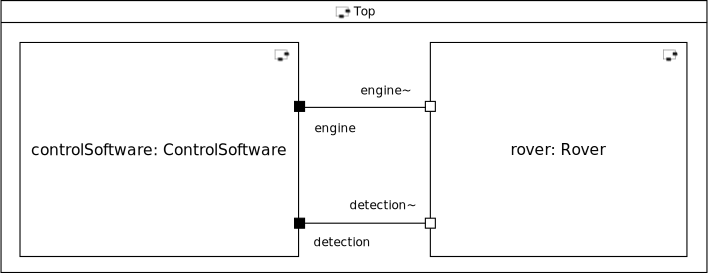
\includegraphics[width=\textwidth]{toplevel}
  \end{center}

  \begin{itemize}
  \item \structure{Capsules}: pretty much components as you know them
  \item Capsule \structure{ports} exchange messages using \structure{protocols}
  \item Here, the program is divided into a control algorithm and an abstraction of the rover hardware
  \end{itemize}
\end{frame}

\begin{frame}{Protocols for capsule communication}
  \begin{center}
    \includegraphics[width=.8\textwidth]{engineprotocol}
  \end{center}

  \begin{itemize}
  \item ``Out'' messages: black port $\rightarrow$ white (``conjugated'') port
  \item ``In'' messages go the other way
  \item Out messages are commands, in messages are notifications
  \end{itemize}
\end{frame}

\begin{frame}{Rover capsule}
  \begin{center}
    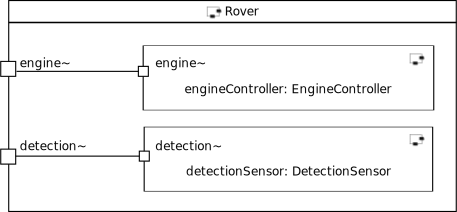
\includegraphics[width=.9\textwidth]{rovercapsule}
  \end{center}

  \begin{itemize}
  \item You can nest capsules inside others
  \item ``Rover'' contains ``EngineController'' and ``DetectionSensor''
  \item Inner capsules handle messages from the ``Rover'' ports
  \end{itemize}

\end{frame}

\begin{frame}{State machine for the ``ControlSoftware'' capsule}
  \framesubtitle{Capsules can have behaviour associated to them through state machines}

  \begin{center}
    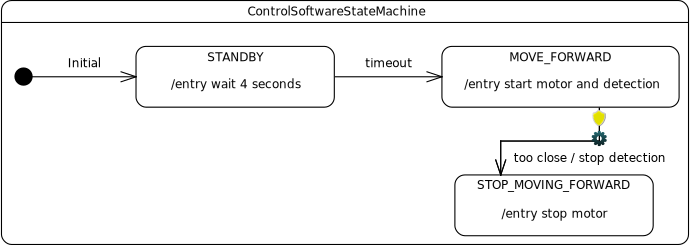
\includegraphics[width=.9\textwidth]{simple-statemachine}
  \end{center}
  \begin{tikzpicture}[overlay,remember picture]
    \begin{scope}[color=red,very thick]
      \draw<2> (page cs:-.65,.5) rectangle (page cs:0,.275);
      \draw<3> (page cs:0,.5) rectangle (page cs:.75,.275);
      \draw<4> (page cs:.3,.3) rectangle (page cs:.75,.1);
      \draw<5> (page cs:.225,.124) rectangle (page cs:.7,-.1);
    \end{scope}
  \end{tikzpicture}\vspace{-2.5em}
  \begin{overprint}
    \onslide<1>
    \begin{itemize}
    \item Same notation as plain UML state machines
      % shallow history, terminate node
    \item Some UML state machine elements are not available
    \item In Papyrus-RT, guards are yellow shields, and gears are effects
    \item Labels only for readability: all behaviour is in C++ snippets
    \end{itemize}
    \onslide<2->
    \begin{enumerate}
    \item \highlight<2>{Asks ``timer'' system service for notification in 4 seconds}
    \item<3-> \highlight<3>{Transitions into ``MOVE\_FORWARD'', asking the
      ``Rover'' capsule to ``goForward'' and ``startDetection''}
    \item<4-> \highlight<4>{``DetectionSensor'' sends ``obstacleDetected'' messages periodically:
      when too close, controller stops detection and transitions into
      ``STOP\_MOVING\_FORWARD''}
    \item<5-> \highlight<5>{Upon entering that state, motor is told to stop}
    \end{enumerate}
  \end{overprint}
\end{frame}

\begin{frame}{State machine for the ``EngineController'' capsule}
  \begin{center}
    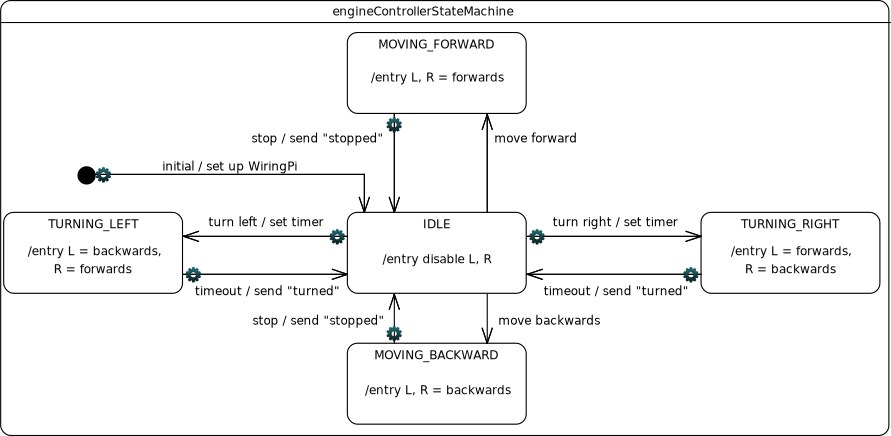
\includegraphics[width=\textwidth]{engine-statemachine}
  \end{center}
  \begin{tikzpicture}[overlay,remember picture]
    \begin{scope}[color=red,very thick]
      \draw<1> (page cs:-.6,.25) rectangle (page cs:-.2,.175);
      \draw<1> (page cs:-.2,.125) rectangle (page cs:.17,-.11);
      \draw<2> (page cs:-.38,.58) rectangle (page cs:.27,.27);
      \draw<2> (page cs:-.38,-.14) rectangle (page cs:.3,-.44);
      \draw<3> (page cs:-.84,.13) rectangle (page cs:-.19,-.12);
      \draw<3> (page cs:.15,.13) rectangle (page cs:.83,-.12);
    \end{scope}
  \end{tikzpicture}\vspace{-2em}
  \begin{itemize}
  \item \highlight<1>{Starts at the IDLE state after setting up the GPIO pins}
  \item<2-> \highlight<2>{Goes forwards/backwards until told to stop, which it confirms}
  \item<3-> \highlight<3>{A timer turns the rover for duration proportional to angle (!)}
  \end{itemize}
\end{frame}


\begin{frame}
  \begin{center}
    \vspace{\stretch{1}}

    \Large Demo time!

    \vspace{\stretch{1}}

    Let's see how it's done with Papyrus-RT, and run the simple state machine in the rover.

    \vspace{\stretch{1}}

  \end{center}
\end{frame}

\section{Exercises}

\begin{frame}{Exercise: make the rover back up and rotate}

  \begin{columns}
    \column{.49\textwidth}

    Modify the ``ControlAlgorithm'' state machine. After
    getting too close and stopping, it should:

    \begin{enumerate}
    \item Wait 2 seconds
    \item Go backwards for 1 second
    \item Turn right 138 degrees
    \item Stop
    \item Go forward again
    \end{enumerate}

    Do it first in English, then think of the messages you should be sending and
    triggering on.

    \column{.51\textwidth}
    \begin{block}{Engine protocol}
      \begin{itemize}
      \item out moveForward()
      \item out moveBackward()
      \item out stop()
      \item out turnLeft(angle)
      \item out turnRight(angle)
      \item in stopped()
      \item in turnedLeft()
      \item in turnedRight()
      \end{itemize}
    \end{block}

    \begin{block}{Timer protocol}
      \begin{itemize}
      \item out informIn(secs, nanosecs)
      \item in timeout()
      \end{itemize}
    \end{block}

  \end{columns}

\end{frame}

\begin{frame}{Solution for the exercise}

  \begin{center}
    \includegraphics[width=\textwidth]{backup-statemachine}
  \end{center}

\end{frame}

\begin{frame}
  \begin{center}
    \vspace{\stretch{1}}

    \Large Demo time again!

    \vspace{\stretch{1}}

    Let's switch to the branch with this solution and try it out on the rover.

    \vspace{\stretch{1}}
  \end{center}
\end{frame}

\begin{frame}{Exercise: how would you improve the rover?}

  \begin{block}{Problems with the latest model}
    \begin{itemize}
    \item Turning angle is fixed, regardless of obstacle
    \item Speed is also fixed, regardless of distance
    \item We are limited by having only one sensor
    \end{itemize}
  \end{block}

  \pause

  \begin{block}{In groups}
    \begin{itemize}
    \item Come up with an idea to improve the rover's behaviour
    \item You can change the protocols if you like
    \item You can add extra ultrasonic range finders, too
      \begin{itemize}
      \item Where would you put them, though?
      \end{itemize}
    \item How would you implement your idea in UML-RT?
    \end{itemize}
  \end{block}

\end{frame}

\begin{frame}
  \begin{center}
    \vspace{\stretch{1}}

    \Large One last demo!

    \vspace{\stretch{1}}

    We have one branch where speed is regulated by the distance to the obstacle,
    and we turn until the obstacle is far enough. Let's try it out.

    \vspace{\stretch{1}}
  \end{center}
\end{frame}

\begin{frame}{In closing}

  \begin{block}{Models can provide useful abstractions}
    \begin{itemize}
    \item With UML-RT, we think about real-time control differently
    \item Collaborating state machines \emph{vs} manual multithreaded coding
    \item The models become C++ code, which we can run on the Pi
    \item This is within the wider area of \alert{executable modelling}
    \end{itemize}
  \end{block}

  \pause

  \begin{block}{Papyrus-RT: your thoughts?}
    \begin{itemize}
    \item Con: it's not as easy as just drawing
    \item Pro: \alert{we can do more things with these models}
    \item Roadmap: sequence/class/activity diagrams
    \item Generating code for other languages is also planned
    \end{itemize}
  \end{block}

\end{frame}

\begin{frame}{Hope you enjoyed it!}
  \centering
  \vspace{\stretch{1}}

  {\Huge Questions? Feedback?}

  \vspace{\stretch{1}}

  Source code for slides and models:\\
  \url{https://github.com/bluezio/rover-demo}

  \vspace{\stretch{1}}

  Step-by-step instructions from scratch here:\\
  \url{https://goo.gl/1jeJ8w}

  %% \twitter{antoniogado}

  \vspace{\stretch{1}}
\end{frame}

% might want to prepare extra slides here
\backupbegin

\begin{frame}{Bibliography}

  \begin{thebibliography}{40}
    \bibitem[UML-RT]{selic06}
    B.~Selic.
    \newblock Using UML for modeling complex real-time systems.
    \newblock Languages, Compilers, and Tools for Embedded Systems, LNCS vol.\ 1474, pp.\ 250--260.
    \newblock {\small\url{https://link.springer.com/chapter/10.1007/BFb0057795}}

  \end{thebibliography}

\end{frame}

\backupend

\end{document}
